%&tex

\documentclass{beamer}

\usepackage[english]{babel}
\usepackage[utf8]{inputenc}
\usepackage{mathtools}
\usepackage{amsthm}
\usepackage{amssymb}
\usepackage{thmtools,thm-restate}
\usepackage{amsfonts}
\usepackage{hyperref}
\usepackage[singlelinecheck=false]{caption}
\usepackage[backend=biber,url=true,doi=true,eprint=false,style=authoryear]{biblatex}
\usepackage{algorithm}
\usepackage[noend]{algpseudocode}
\usepackage{listings}
\usepackage{subcaption}
\usepackage{xcolor}

\usepackage{graphicx}
\usepackage{tikz}
\usetikzlibrary{positioning}
\usetikzlibrary{shapes.geometric}
\usetikzlibrary{fit}
\usetikzlibrary{calc}

\usepackage{tkz-graph}

\addbibresource{references.bib}
\usetheme{metropolis}

\DeclareMathOperator*{\argmin}{arg\,min}
\DeclareMathOperator*{\argmax}{arg\,max}
\DeclareMathOperator*{\Val}{\text{Val}}
\DeclareMathOperator*{\Ch}{\text{Ch}}
\DeclareMathOperator*{\Pa}{\text{Pa}}
\DeclareMathOperator*{\Sc}{\text{Sc}}
\newcommand{\ov}{\overline}
\newcommand{\tsup}{\textsuperscript}

\newcommand\defeq{\mathrel{\overset{\makebox[0pt]{\mbox{\normalfont\tiny\sffamily def}}}{=}}}

\newcommand{\algorithmautorefname}{Algorithm}
\algrenewcommand\algorithmicrequire{\textbf{Input}}
\algrenewcommand\algorithmicensure{\textbf{Output}}
\algnewcommand{\LineComment}[1]{\State\,\(\triangleright\) #1}

\newcommand{\Left}{\text{LEFT}}
\newcommand{\Right}{\text{RIGHT}}
\newcommand{\Up}{\text{UP}}

\newcommand{\set}[1]{\mathbf{#1}}
\newcommand{\pr}{\text{P}}
\newcommand{\eps}{\varepsilon}
\newcommand{\ddspn}[2]{\frac{\partial#1}{\partial#2}}
\newcommand{\iddspn}[2]{\partial#1/\partial#2}
\newcommand{\indep}{\perp}
\renewcommand{\implies}{\Rightarrow}

\newcommand{\bigo}{\mathcal{O}}
\newcommand{\mbf}[1]{\mathbf{#1}}

\setbeamertemplate{theorems}[ams style]

\setbeamersize{description width=1.0cm}

\lstset{frameround=fttt,
	numbers=left,
	breaklines=true,
	keywordstyle=\bfseries,
	basicstyle=\ttfamily,
}

\newcommand{\code}[1]{\lstinline[mathescape=true]{#1}}
\newcommand{\mcode}[1]{\lstinline[mathescape]!#1!}

\title{Learning Sum-Product Networks}
\date{}
\author{Renato Lui Geh}
\institute{Institute of Mathematics and Statistics --- University of São Paulo}

\begin{document}

\maketitle

\section{Introduction}

\begin{frame}
  \frametitle{Definition}
  \begin{definition}[Generalized sum-product network]~\\
    A sum-product network (SPN) is a DAG where each node $n$ is either:
    \begin{enumerate}
      \item A tractable univariate probability distribution;
      \item A product of SPNs: $v_n=\prod_{j\in\Ch(n)}v_j$; or
      \item A weighted sum of SPNs: $v_n=\sum_{j\in\Ch(n)}w_{n,j}v_j$.
    \end{enumerate}
    Where $v_n$ is the value of node $n$, $\Ch(n)$ its set of children and $w_{n,j}$ the weight of
    edge $n\to j$.
  \end{definition}
\end{frame}

\begin{frame}
  \frametitle{Scope}

  The scope $\Sc(n)$ of node $n$ is the union of the scope of its children. The scope of a leaf is
  the set of all variables in the distribution. Let $S$ be the root of the SPN below:
  \vspace{-0.75cm}

  \begin{center}
    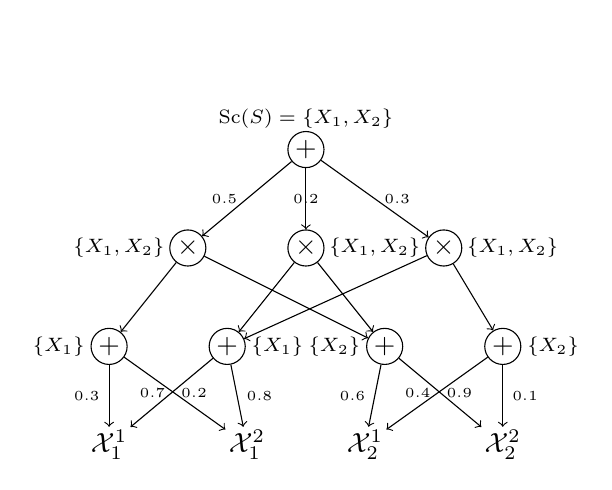
\begin{tikzpicture}
      \begin{scope}[every node/.style={circle,draw,inner sep=1pt}]
        \node[label={[label distance=-1.0cm]above:{\scriptsize$\Sc(S)=\{X_1,X_2\}$}}] (root) at (0, 0) {+};
        \node[label=left:{\scriptsize$\{X_1,X_2\}$}] (p1) at (-1.5, -1.25) {$\times$};
        \node[label=right:{\scriptsize$\{X_1,X_2\}$}] (p2) at (0, -1.25) {$\times$};
        \node[label=right:{\scriptsize$\{X_1,X_2\}$}] (p3) at (1.75, -1.25) {$\times$};
        \node[label=left:\scriptsize$\{X_1\}$] (s1) at (-2.5, -2.5) {+};
        \node[label=right:\scriptsize$\{X_1\}$] (s2) at (-1.0, -2.5) {+};
        \node[label=left:\scriptsize$\{X_2\}$] (s3) at (1.0, -2.5) {+};
        \node[label=right:\scriptsize$\{X_2\}$] (s4) at (2.5, -2.5) {+};
        \node[draw=none,fill=none,rectangle] (x11) at (-2.5, -3.75) {$\mathcal{X}_1^1$};
        \node[draw=none,fill=none,rectangle] (x12) at (-0.75, -3.75) {$\mathcal{X}_1^2$};
        \node[draw=none,fill=none,rectangle] (x21) at (0.75, -3.75) {$\mathcal{X}_2^1$};
        \node[draw=none,fill=none,rectangle] (x22) at (2.5, -3.75) {$\mathcal{X}_2^2$};
      \end{scope}

      \begin{scope}[every path/.style={->}]
        \draw (root) -- node[left]{\tiny$0.5$} (p1);
        \draw (root) -- node{\tiny$0.2$} (p2);
        \draw (root) -- node[right]{\tiny$0.3$} (p3);
        \draw (p1) -- (s1);
        \draw (p1) -- (s3);
        \draw (p2) -- (s2);
        \draw (p2) -- (s3);
        \draw (p3) -- (s2);
        \draw (p3) -- (s4);
        \draw (s1) -- node[left]{\tiny$0.3$} (x11);
        \draw (s1) -- node[left]{\tiny$0.7$} (x12);
        \draw (s2) -- node[right]{\tiny$0.2$} (x11);
        \draw (s2) -- node[right]{\tiny$0.8$} (x12);
        \draw (s3) -- node[left]{\tiny$0.6$} (x21);
        \draw (s3) -- node[left]{\tiny$0.4$} (x22);
        \draw (s4) -- node[right]{\tiny$0.9$} (x21);
        \draw (s4) -- node[right]{\tiny$0.1$} (x22);
      \end{scope}
    \end{tikzpicture}
  \end{center}

\end{frame}

\begin{frame}
  \frametitle{Validity}

  \begin{definition}[Validity]~\\
    Let $S$ be an SPN. If $S$ correctly computes and marginalizes an unnormalized probability
    $\phi(\mbf{X})$, then it is said to be \emph{valid}.
  \end{definition}~\\

  If for every sum node $n$

  \begin{equation*}
    \forall j\in\Ch(n), w_{n,j} \geq 0\text{ and }\sum_{j\in\Ch(n)}w_{n,j} = 1
  \end{equation*}

  then $S$ represents the probability distribution itself.\\~\\

  A \textbf{sufficient}, yet not necessary, condition for validity is \emph{completeness} and
  \emph{consistency} (\cite{poon-domingos}).

\end{frame}

\begin{frame}
  \frametitle{Completeness}
  \begin{definition}[Completeness]~\\
    An SPN $S$ is said to be complete, iff for each sum node $s\in S$, all children of $s$ have
    same scope.
  \end{definition}
  \vspace{-0.5cm}

  \begin{center}
    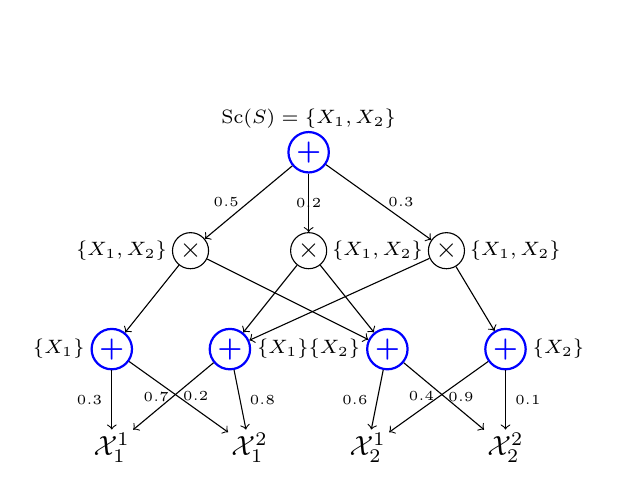
\begin{tikzpicture}
      \begin{scope}[every node/.style={circle,draw,inner sep=1pt}]
        \node[color=blue,thick,label={[label
          distance=-1.0cm]above:{\scriptsize$\Sc(S)=\{X_1,X_2\}$}}] (root) at (0, 0) {\textbf{+}};
        \node[label=left:{\scriptsize$\{X_1,X_2\}$}] (p1) at (-1.5, -1.25) {$\times$};
        \node[label=right:{\scriptsize$\{X_1,X_2\}$}] (p2) at (0, -1.25) {$\times$};
        \node[label=right:{\scriptsize$\{X_1,X_2\}$}] (p3) at (1.75, -1.25) {$\times$};
        \node[color=blue,thick,label=left:\scriptsize$\{X_1\}$] (s1) at (-2.5, -2.5) {\textbf{+}};
        \node[color=blue,thick,label=right:\scriptsize$\{X_1\}$] (s2) at (-1.0, -2.5) {\textbf{+}};
        \node[color=blue,thick,label=left:\scriptsize$\{X_2\}$] (s3) at (1.0, -2.5) {\textbf{+}};
        \node[color=blue,thick,label=right:\scriptsize$\{X_2\}$] (s4) at (2.5, -2.5) {\textbf{+}};
        \node[draw=none,fill=none,rectangle] (x11) at (-2.5, -3.75) {$\mathcal{X}_1^1$};
        \node[draw=none,fill=none,rectangle] (x12) at (-0.75, -3.75) {$\mathcal{X}_1^2$};
        \node[draw=none,fill=none,rectangle] (x21) at (0.75, -3.75) {$\mathcal{X}_2^1$};
        \node[draw=none,fill=none,rectangle] (x22) at (2.5, -3.75) {$\mathcal{X}_2^2$};
      \end{scope}

      \begin{scope}[every path/.style={->}]
        \draw (root) -- node[left]{\tiny$0.5$} (p1);
        \draw (root) -- node{\tiny$0.2$} (p2);
        \draw (root) -- node[right]{\tiny$0.3$} (p3);
        \draw (p1) -- (s1);
        \draw (p1) -- (s3);
        \draw (p2) -- (s2);
        \draw (p2) -- (s3);
        \draw (p3) -- (s2);
        \draw (p3) -- (s4);
        \draw (s1) -- node[left]{\tiny$0.3$} (x11);
        \draw (s1) -- node[left]{\tiny$0.7$} (x12);
        \draw (s2) -- node[right]{\tiny$0.2$} (x11);
        \draw (s2) -- node[right]{\tiny$0.8$} (x12);
        \draw (s3) -- node[left]{\tiny$0.6$} (x21);
        \draw (s3) -- node[left]{\tiny$0.4$} (x22);
        \draw (s4) -- node[right]{\tiny$0.9$} (x21);
        \draw (s4) -- node[right]{\tiny$0.1$} (x22);
      \end{scope}
    \end{tikzpicture}
  \end{center}
\end{frame}

\begin{frame}
  \frametitle{Consistency}
  \begin{definition}[Consistency]~\\
    An SPN $S$ is said to be consistent, iff no variable appears with a value $v$ in one child of a
    product node, and valued $u$, with $u\neq v$, in another.
  \end{definition}

  \begin{center}
    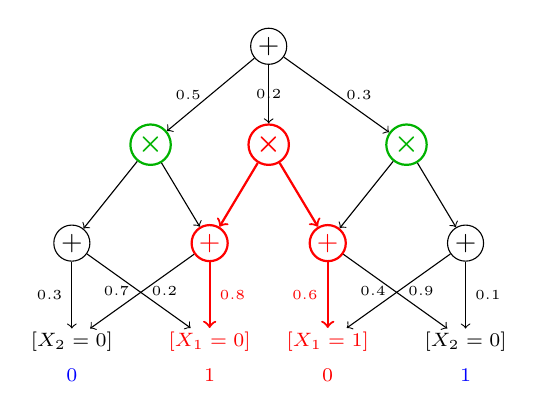
\begin{tikzpicture}
      \begin{scope}[every node/.style={circle,draw,inner sep=1pt}]
        \node (root) at (0, 0) {+};
        \node[color=black!30!green,thick] (p1) at (-1.5, -1.25) {$\boldsymbol{\times}$};
        \node[color=red,thick] (p2) at (0, -1.25) {$\boldsymbol{\times}$};
        \node[color=black!30!green,thick] (p3) at (1.75, -1.25) {$\boldsymbol{\times}$};
        \node (s1) at (-2.5, -2.5) {+};
        \node[color=red,thick] (s2) at (-0.75, -2.5) {+};
        \node[color=red,thick] (s3) at (0.75, -2.5) {+};
        \node (s4) at (2.5, -2.5) {+};
        \node[label={[label
          distance=0.1cm,color=blue]below:{\scriptsize$0$}},draw=none,fill=none,rectangle] (x11) at
          (-2.5, -3.75) {\scriptsize$[X_2=0]$};
        \node[color=red,thick,label={[label
          distance=0.1cm,color=red]below:{\scriptsize$1$}},draw=none,fill=none,rectangle] (x12) at
          (-0.75, -3.75) {\scriptsize$[X_1=0]$};
        \node[color=red,thick,label={[label
          distance=0.1cm,color=red]below:{\scriptsize$0$}},draw=none,fill=none,rectangle] (x21) at
          (0.75, -3.75) {\scriptsize$[X_1=1]$};
        \node[label={[label
          distance=0.1cm,color=blue]below:{\scriptsize$1$}},draw=none,fill=none,rectangle] (x22) at
          (2.5, -3.75) {\scriptsize$[X_2=0]$};
      \end{scope}

      \begin{scope}[every path/.style={->}]
        \draw (root) -- node[left]{\tiny$0.5$} (p1);
        \draw (root) -- node{\tiny$0.2$} (p2);
        \draw (root) -- node[right]{\tiny$0.3$} (p3);
        \draw (p1) -- (s1);
        \draw (p1) -- (s2);
        \draw[thick,color=red] (p2) -- (s2);
        \draw[thick,color=red] (p2) -- (s3);
        \draw (p3) -- (s3);
        \draw (p3) -- (s4);
        \draw (s1) -- node[left]{\tiny$0.3$} (x11);
        \draw (s1) -- node[left]{\tiny$0.7$} (x12);
        \draw (s2) -- node[right]{\tiny$0.2$} (x11);
        \draw[thick,color=red] (s2) -- node[right]{\tiny$0.8$} (x12);
        \draw[thick,color=red] (s3) -- node[left]{\tiny$0.6$} (x21);
        \draw (s3) -- node[left]{\tiny$0.4$} (x22);
        \draw (s4) -- node[right]{\tiny$0.9$} (x21);
        \draw (s4) -- node[right]{\tiny$0.1$} (x22);
      \end{scope}
    \end{tikzpicture}
  \end{center}\vspace{-1.0cm}

  \begin{equation*}
    X=\{X_1=0,X_2=1\}
  \end{equation*}

\end{frame}

\begin{frame}
  \frametitle{Decomposability}

  \begin{definition}[Decomposability]~\\
    An SPN is decomposable iff no variable appears in more than one child of a product node (i.e.
    scopes are disjoint).
  \end{definition}\vspace{-0.5cm}

  \begin{center}
    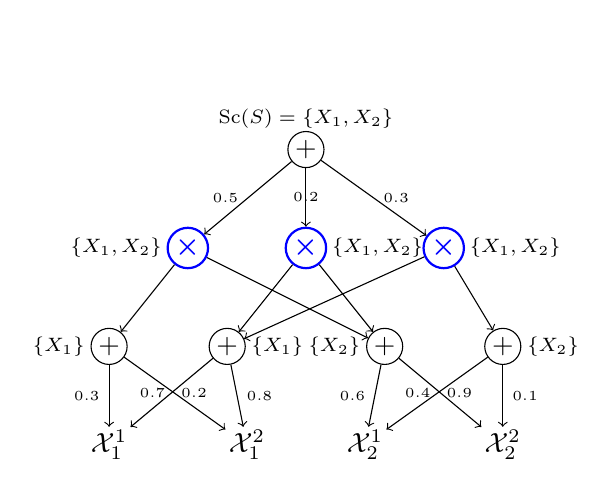
\begin{tikzpicture}
      \begin{scope}[every node/.style={circle,draw,inner sep=1pt}]
        \node[label={[label distance=-1.0cm]above:{\scriptsize$\Sc(S)=\{X_1,X_2\}$}}] (root) at (0, 0) {+};
        \node[color=blue,thick,label=left:{\scriptsize$\{X_1,X_2\}$}] (p1) at (-1.5, -1.25)
          {$\boldsymbol{\times}$};
        \node[color=blue,thick,label=right:{\scriptsize$\{X_1,X_2\}$}] (p2) at (0, -1.25)
          {$\boldsymbol{\times}$};
        \node[color=blue,thick,label=right:{\scriptsize$\{X_1,X_2\}$}] (p3) at (1.75, -1.25)
          {$\boldsymbol\times$};
        \node[label=left:\scriptsize$\{X_1\}$] (s1) at (-2.5, -2.5) {+};
        \node[label=right:\scriptsize$\{X_1\}$] (s2) at (-1.0, -2.5) {+};
        \node[label=left:\scriptsize$\{X_2\}$] (s3) at (1.0, -2.5) {+};
        \node[label=right:\scriptsize$\{X_2\}$] (s4) at (2.5, -2.5) {+};
        \node[draw=none,fill=none,rectangle] (x11) at (-2.5, -3.75) {$\mathcal{X}_1^1$};
        \node[draw=none,fill=none,rectangle] (x12) at (-0.75, -3.75) {$\mathcal{X}_1^2$};
        \node[draw=none,fill=none,rectangle] (x21) at (0.75, -3.75) {$\mathcal{X}_2^1$};
        \node[draw=none,fill=none,rectangle] (x22) at (2.5, -3.75) {$\mathcal{X}_2^2$};
      \end{scope}

      \begin{scope}[every path/.style={->}]
        \draw (root) -- node[left]{\tiny$0.5$} (p1);
        \draw (root) -- node{\tiny$0.2$} (p2);
        \draw (root) -- node[right]{\tiny$0.3$} (p3);
        \draw (p1) -- (s1);
        \draw (p1) -- (s3);
        \draw (p2) -- (s2);
        \draw (p2) -- (s3);
        \draw (p3) -- (s2);
        \draw (p3) -- (s4);
        \draw (s1) -- node[left]{\tiny$0.3$} (x11);
        \draw (s1) -- node[left]{\tiny$0.7$} (x12);
        \draw (s2) -- node[right]{\tiny$0.2$} (x11);
        \draw (s2) -- node[right]{\tiny$0.8$} (x12);
        \draw (s3) -- node[left]{\tiny$0.6$} (x21);
        \draw (s3) -- node[left]{\tiny$0.4$} (x22);
        \draw (s4) -- node[right]{\tiny$0.9$} (x21);
        \draw (s4) -- node[right]{\tiny$0.1$} (x22);
      \end{scope}
    \end{tikzpicture}
  \end{center}
\end{frame}

\begin{frame}
  \frametitle{Decomposability vs Consistency}

  \textbf{Decomposability} implies \textbf{consistency}.
  \vfill

  But \textbf{decomposability} is much easier for learning, and allows for an interpretation of
  product nodes as \emph{independencies} between variables.
  \vfill

  \cite{theoretical-spn} shows \textbf{decomposable} SPNs are as representable as solely
  \textbf{consistent} ones.
\end{frame}


\section{Learning}

\begin{frame}
  \frametitle{Learning types}

  Two main types of learning:

  \begin{description}
    \item[Structure learning:]~\\
      Learn graph structure from data.
    \item[Parameter learning:]~\\
      Learn weights from data given a fixed graph structure.
  \end{description}

  Both usually attempt to optimize log-likelihood.

\end{frame}

\begin{frame}
  \frametitle{Structure learning}

  \begin{itemize}
    \item Structure learning:
      \begin{enumerate}
        \item \textbf{Poon-Domingos dense architecture}~(\cite{poon-domingos});
        \item \textbf{Gens-Domingos LearnSPN}~(\cite{gens-domingos});
        \item \textbf{Dennis-Ventura clustering architecture}~(\cite{clustering});
        \item \textbf{Random Tensorized SPNs (RAT-SPNs)}~(\cite{deep-learn-spn});
        \item Indirect-Direct SPNs (ID-SPNs)~(\cite{id-spn});
        \item LearnSPN+Chow-Liu Trees (LearnSPN-BTB)~(\cite{vergari-mauro}).
      \end{enumerate}
  \end{itemize}

\end{frame}

\begin{frame}
  \frametitle{Parameter learning}

  \begin{itemize}
    \item Parameter learning:
      \begin{enumerate}
        \item \textbf{Generative Gradient Descent}~(\cite{poon-domingos,diff-approach-darwiche});
        \item \textbf{Discriminative Gradient Descent}~(\cite{discriminative});
        \item Expectation-Maximization~(\cite{poon-domingos});
        \item Extended Baum-Welch~(\cite{baum-welch});
        \item Collapsed Variational Inference~(\cite{variational-spn});
        \item Bayesian Moment Matching~(\cite{bayesian-moment}).
      \end{enumerate}
  \end{itemize}
\end{frame}

\section{Parameter learning}

\begin{frame}
  \frametitle{Generative vs Discriminative Gradient Descent}

  \begin{description}
    \item[Generative:]~\\
      \begin{itemize}
        \item Optimize log-likelihood of $P(X,Y)$
        \item Gradient: $\ddspn{}{W}\log P(X,Y)$
        \item E.g. completion
      \end{itemize}
    \item[Discriminative:]~\\
      \begin{itemize}
        \item Optimize log-likelihood of $P(Y|X)$
        \item Gradient: $\ddspn{}{W}\log P(Y|X)$
        \item E.g. classification
      \end{itemize}
  \end{description}

  \centering{\textbf{Generative} representation is able to extract its \textbf{discriminative}.}

  \begin{equation*}
    P(Y|X)=\frac{P(X,Y)}{P(Y)}
  \end{equation*}
\end{frame}

\begin{frame}
  \frametitle{Derivatives I}

  Let $S$ be an SPN, and $W$ the set of weights of $S$. Denote by $S_n$ the sub-SPN rooted at node
  $n$.

  \centering{\textbf{Objective:} find gradient $\ddspn{}{W}\log S$.}

  That is, compute each component $\iddspn{S}{w_{n,j}}$, for each edge $n\to j$.

  \begin{align*}
    \ddspn{S}{w_{n,j}}(X)&=\ddspn{S}{S_n}\ddspn{S_n}{w_{n,j}}(X)\\
      &=\ddspn{S}{S_n}\ddspn{}{w_{n,j}}\left(\sum_{i\in\Ch(n)}w_{n,i}S_i(X)\right)\\
      &=\ddspn{S}{S_n}S_j(X).
  \end{align*}

  We now need to find a form for derivative $\ddspn{S}{S_n}$.
\end{frame}

\begin{frame}
  \frametitle{Derivatives II}

  Let's find the sub-SPN derivative $\ddspn{S}{S_j}$. From chain rule:

  \begin{align*}
    \ddspn{S}{S_j}(X)&=\sum_{n\in\Pa(j)}\ddspn{S}{S_n}\ddspn{S_n}{S_j}(X)\\
      &=\underbrace{\sum_{\substack{n\in\Pa(j)\\n:\text{
        sum}}}\ddspn{S}{S_n}\ddspn{S_n}{S_j}(X)}_{(\ast)}+
      \underbrace{\sum_{\substack{n\in\Pa(j)\\n:\text{
        product}}}\ddspn{S}{S_n}\ddspn{S_n}{S_j}(X)}_{(\ast\ast)}
  \end{align*}

  Let's analyze two cases: when $n$ is a sum node $(\ast)$, and when it's a product node
  $(\ast\ast)$.
\end{frame}

\begin{frame}
  \frametitle{Derivatives III}

  \textbf{Case 1:} when $n$ is a sum node.

  \begin{align*}
    (\ast)&=\sum_{\substack{n\in\Pa(j)\\n:\text{ sum}}}\ddspn{S}{S_n}\ddspn{S_n}{S_j}(X)\\
          &=\sum_{\substack{n\in\Pa(j)\\n:\text{ sum}}}\ddspn{S}{S_n}\ddspn{}{S_j}\left(\sum_{i\in\Ch(n)}
    w_{n,i}S_i(X)\right)\\
          &=\sum_{\substack{n\in\Pa(j)\\n:\text{ sum}}}\ddspn{S}{S_n}w_{n,j}
  \end{align*}
\end{frame}

\begin{frame}
  \frametitle{Derivatives IV}

  \textbf{Case 2:} when $n$ is a product node.

  \begin{align*}
    (\ast\ast)&=\sum_{\substack{n\in\Pa(j)\\n:\text{ product}}}\ddspn{S}{S_n}\ddspn{S_n}{S_j}(X)\\
      &=\sum_{\substack{n\in\Pa(j)\\n:\text{ product}}}\ddspn{S}{S_n}\ddspn{}{S_j}\left(\prod_{i\in\Ch(n)}
      S_i(X)\right)\\
      &=\sum_{\substack{n\in\Pa(j)\\n:\text{ product}}}\ddspn{S}{S_n}\prod_{k\in
      \Ch(n)\setminus\{j\}}S_k
  \end{align*}
\end{frame}

\begin{frame}
  \frametitle{Derivatives V}

  Going back to our original formula and using the derived forms of $(\ast)$ and $(\ast\ast)$:

  \begin{align*}
    \ddspn{S}{S_j}(X)&=\sum_{\substack{n\in\Pa(j)\\n:\text{
          sum}}}\ddspn{S}{S_n}\ddspn{S_n}{S_j}(X)&+&\sum_{\substack{n\in\Pa(j)\\n:\text{
      product}}}\ddspn{S}{S_n}\ddspn{S_n}{S_j}(X)\\
                     &=\sum_{\substack{n\in\Pa(j)\\n:\text{
          sum}}}\ddspn{S}{S_n}w_{n,j}&+&\sum_{\substack{n\in\Pa(j)\\n:\text{
                       product}}}\ddspn{S}{S_n}\prod_{k\in \Ch(n)\setminus\{j\}}S_k
  \end{align*}

  \begin{center}
    \textbf{Remark:} when $j$ is the root node: $\ddspn{S}{S_j}=\ddspn{S}{S}=1$.
  \end{center}

  The above form lends itself nicely to an algorithmic format.
\end{frame}

\begin{frame}
  \frametitle{Derivatives VI}

  \begin{algorithm}[H]
    \caption{\code{Backprop}: Backpropagation derivation on SPNs}
    \begin{algorithmic}[1]
      \Require A valid SPN $S$ with pre-computed probabilities $S_n(X)$
      \Ensure Partial derivatives of $S$ with respect to every node and weight
      \State Initialize $\ddspn{S}{S_n}=0$ except $\ddspn{S}{S}=1$
      \For{each node $n\in S$ in top-down order}
        \If{$n$ is sum node}
          \For{all $j\in\Ch(n)$}
            \State $\ddspn{S}{S_j}\gets\ddspn{S}{S_j}+w_{n,j}\ddspn{S}{S_n}$
            \State $\ddspn{S}{w_{n,j}}\gets\ddspn{S}{S_n}S_j$
          \EndFor%
        \Else%
          \For{all $j\in\Ch(n)$}
            \State $\ddspn{S}{S_j}\gets\ddspn{S}{S_j}+\ddspn{S}{S_n}\prod_{k\in\Ch(n)\setminus
              \{j\}}S_k$
          \EndFor%
        \EndIf
      \EndFor%
    \end{algorithmic}
  \end{algorithm}
\end{frame}

\begin{frame}
  \frametitle{Generative gradient descent}

  Let's go back to our original objective of finding the gradient. For the \textbf{generative}
  (joint distribution) case:

  \begin{align*}
    \ddspn{}{W}\log P(X,Y)&=\ddspn{}{W}\log S(X,Y)\\
                          &=\frac{1}{S(X,Y)}\ddspn{S}{W}(X,Y)\propto\ddspn{S}{W}(X,Y)
  \end{align*}

  So it is sufficient to find $\ddspn{S}{W}$, which we already have. Our weight update is then:

  \begin{equation*}
    \Delta w_{n,j}=\eta\ddspn{S}{w_{n,j}}(X,Y)
  \end{equation*}
\end{frame}

\begin{frame}
  \frametitle{Discriminative gradient descent}

  For the \textbf{discriminative} (conditional distribution) case:

  \begin{align*}
    \ddspn{}{W}\log P(Y|X)&=\ddspn{}{W}\log\left(\frac{P(Y,X)}{P(X)}\right)\\
                          &=\ddspn{}{W}\log P(Y,X)&-\quad&\ddspn{}{W}\log P(X)\\
                          &=\frac{1}{S(Y,X)}\ddspn{}{W}S(Y,X)&-\quad&\frac{1}{S(X)}\ddspn{}{W}S(X)
  \end{align*}

  Weight updates will take the following form:

  \begin{equation*}
    \Delta w_{n,j}=\eta\left(\frac{1}{S(Y,X)}\ddspn{S(Y,X)}{w_{n,j}}-\frac{1}{S(X)}
      \ddspn{S(X)}{w_{n,j}}\right)
  \end{equation*}

\end{frame}

\begin{frame}
  \frametitle{Soft vs hard derivation}

  Results derived in the previous slides are called \textbf{soft}. Soft gradient means weight
  updates are derivatives of network evaluations. The \textbf{deeper} the network, the
  \textbf{fainter} the signal.

  \begin{figure}[h]
    \centering
    \begin{subfigure}[b]{0.45\linewidth}
      \centering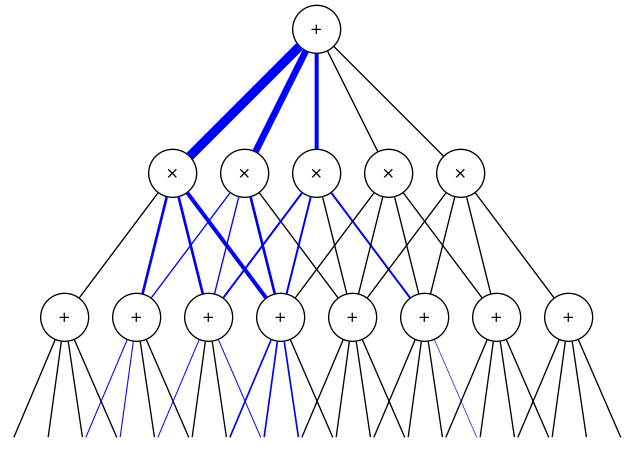
\includegraphics[width=\textwidth]{imgs/softgrad.png}
      \captionsetup{justification=centering}
      \caption{Soft gradient}
    \end{subfigure}
    \begin{subfigure}[b]{0.45\linewidth}
      \centering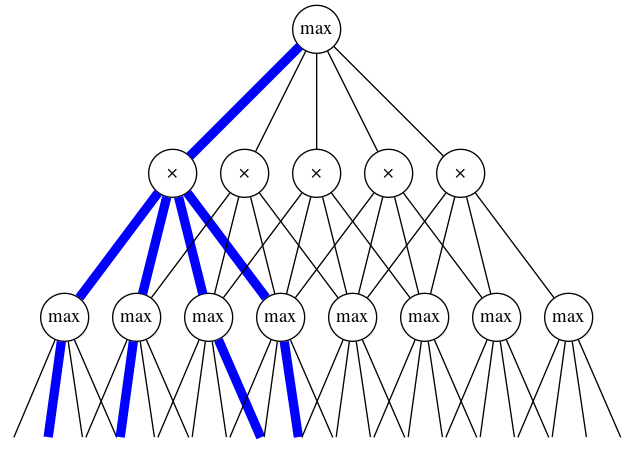
\includegraphics[width=\textwidth]{imgs/hardgrad.png}
      \captionsetup{justification=centering}
      \caption{Hard gradient}
    \end{subfigure}
  \end{figure}

  This is called \textbf{gradient diffusion}. A solution to this is \textbf{hard} gradient descent.
\end{frame}

\begin{frame}
  \frametitle{Hard derivatives I}

  Let $S$ be an SPN. Instead of $\ddspn{S}{W}$, we'll derive $\ddspn{M}{W}$, where $M$ is the
  Max-Product Network (MPN) of $S$. $M$ can be extracted from $S$ by replacing sums with max nodes.

  \begin{description}
    \item[Soft:]~\\
      \begin{itemize}
        \item $\iddspn{S}{W}$
        \item $W$ is the set of weights of $S$
        \item Messages are derivatives
      \end{itemize}
    \item[Hard:]~\\
      \begin{itemize}
        \item $\iddspn{M}{W}$
        \item $W$ is the multiset of weights that a forward pass through $M$ visits
        \item Messages are counts
      \end{itemize}
  \end{description}
\end{frame}

\begin{frame}
  \frametitle{Hard derivatives II}

  \begin{center}
    \textbf{Objective:} find gradient $\ddspn{M}{W}$
  \end{center}

  We know that $M(X)=\prod_{w_i\in W} w_i^{c_i}$, where $c_i$ is the number of times $w_i$ appears
  in $W$. Let's take the logarithm of $M$ on each component:

  \begin{align*}
    \ddspn{\log M}{w_{n,j}}(X)&=\ddspn{}{w_{n,j}}\log\left(\prod_{w_i\in W}w_i^{c_i}\right)\\
                              &=\frac{1}{\prod_{w_i\in W}w_i^{c_i}}\cdot c_{n,j}w_{n,j}^{c_{n,j}-1}
    \cdot\prod_{w_i\in W\setminus\{w_{n,j}\}}w_i^{c_i}\\
                              &=c_{n,j}\frac{w_{n,j}^{c_{n,j}-1}}{w_{n,j}^{c_{n,j}}}
                              =\frac{c_{n,j}}{w_{n,j}}
  \end{align*}
\end{frame}

\begin{frame}
  \frametitle{Hard generative gradient descent}

  From our previous result, we know that:

  \begin{equation*}
    \ddspn{\log M}{w_{n,j}}(X)=\frac{c_{n,j}}{w_{n,j}}
  \end{equation*}

  But that's exactly the log-likelihood for the generative case! This gives us the following weight
  update:

  \begin{equation*}
    \Delta w_{n,j}=\eta\frac{c_{n,j}}{w_{n,j}}
  \end{equation*}

  Note how $c_{n,j}$ is an integer, and $w_{n,j}\in [0,1]$, meaning the signal passed at learning
  does not depend on network size or depth, avoiding the problem of gradient diffusion.
\end{frame}

\begin{frame}
  \frametitle{Hard discriminative gradient descent I}

  For the discriminative case we want:
  \begin{equation*}
    \ddspn{}{W}\log\tilde{P}(Y|X)=\ddspn{}{W}\log\left(\frac{\tilde{P}(Y,X)}{\tilde{P}(X)}\right)=
    \ddspn{}{W}\log\left(\frac{M(Y,X)}{M(X)}\right)
  \end{equation*}

  Where $\tilde{P}$ is the MAP. Apply chain rule:
  \begin{align*}
    \ddspn{}{W}\log\left(\frac{M(Y,X)}{M(X)}\right)&=\ddspn{}{W}\log M(Y,X)-\ddspn{}{W}\log M(X)
  \end{align*}

  For each component:
  \begin{align*}
    \ddspn{}{w_{n,j}}\log\tilde{P}(Y|X)&=\ddspn{}{w_{n,j}}\log M(Y,X)- \ddspn{}{w_{n,j}}\log M(X)\\
                                       &=\ddspn{}{w_{n,j}}c_{n,j}-\ddspn{}{w_{n,j}}\hat{c}_{n,j}\\
                                       &=\frac{\Delta c_{n,j}}{w_{n,j}}
  \end{align*}
\end{frame}

\begin{frame}
  \frametitle{Hard discriminative gradient descent II}

  Visually, $\Delta c_{n,j}$ is the difference between the path of evaluation $M(Y, X)$ and $M(X)$.

  \begin{figure}[h]
    \centering
    \begin{minipage}{0.3\textwidth}
      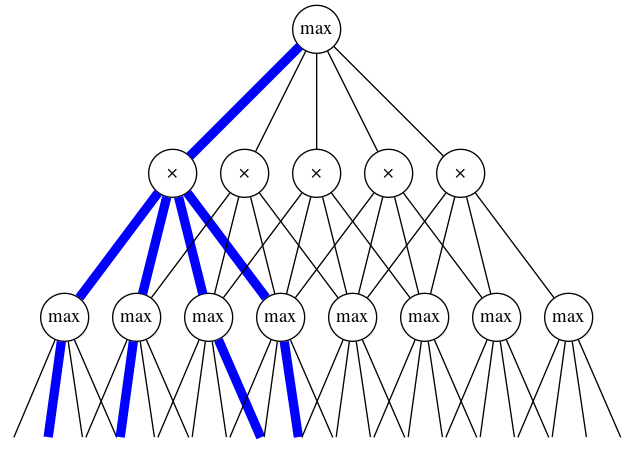
\includegraphics[width=\linewidth]{imgs/hard_diff_0.png}
      \captionsetup{justification=centering}
      \caption*{$\ddspn{}{W}\log M(Y,X)$}
    \end{minipage}
    $-$
    \begin{minipage}{0.3\textwidth}
      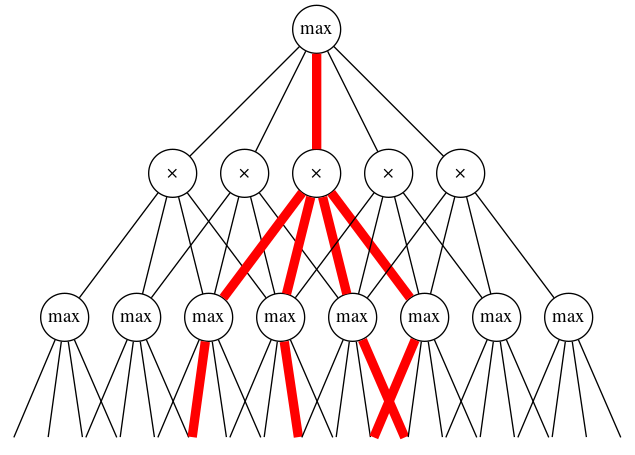
\includegraphics[width=\linewidth]{imgs/hard_diff_1.png}
      \captionsetup{justification=centering}
      \caption*{$\ddspn{}{W}\log M(X)$}
    \end{minipage}
    $=$
    \begin{minipage}{0.3\textwidth}
      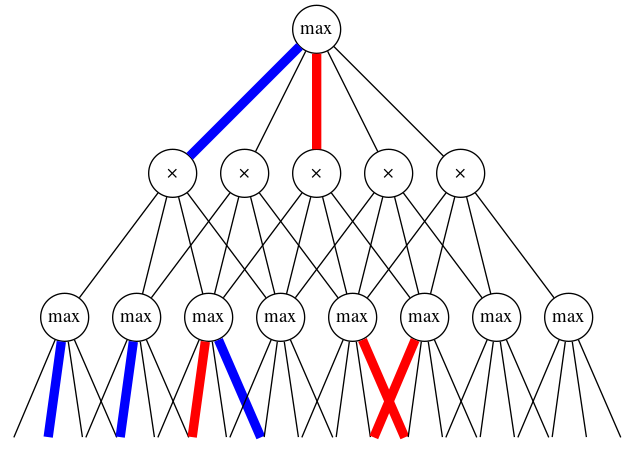
\includegraphics[width=\linewidth]{imgs/hard_diff_2.png}
      \captionsetup{justification=centering}
      \caption*{$\nabla\log\tilde{P}(Y|X)$}
    \end{minipage}
  \end{figure}

  Edges in blue represent positive values, red are negative values and uncolored edges have zero
  value.
\end{frame}

\begin{frame}
  \frametitle{Summary}

  \scriptsize
  \begin{center}\footnotesize\textbf{Generative Gradient Descent}\end{center}\vspace{-0.25cm}
  \begin{table}[h]
    \centering
    \begin{tabular}{l|l}
      \hline
      \multicolumn{1}{c}{\bfseries Inference} & \multicolumn{1}{c}{\bfseries Weight updates}\\
      \hline & \\
      \textbf{Soft} & \(\displaystyle \Delta w_{n,j}=\eta\ddspn{S}{w_{n,j}}(X, Y)\) \\
      & \\
      \textbf{Hard} & \(\displaystyle \Delta w_{n,j}=\eta\frac{c_{n,j}}{w_{n,j}}\) \\
      & \\
      \hline
    \end{tabular}
  \end{table}

  \begin{center}\footnotesize\textbf{Discriminative Gradient Descent}\end{center}\vspace{-0.25cm}
  \begin{table}[h]
    \centering
    \begin{tabular}{l|l}
      \hline
      \multicolumn{1}{c}{\bfseries Inference} & \multicolumn{1}{c}{\bfseries Weight updates}\\
      \hline & \\
      \textbf{Soft} & \(\displaystyle \Delta
        w_{n,j}=\eta\left(\frac{1}{S(Y,X)}\ddspn{S(Y,X)}{w_{n,j}}-\frac{1}{S(X)}
          \ddspn{S(X)}{w_{n,j}}\right)\) \\
      & \\
      \textbf{Hard} & \(\displaystyle \Delta w_{n,j}=\eta\frac{\Delta c_{n,j}}{w_{n,j}}\) \\
      & \\
      \hline
    \end{tabular}
  \end{table}

\end{frame}

\section{Structure learning}

\begin{frame}
\end{frame}


\begin{frame}[standout]
  \textbf{Thank you.\\~\\Questions?}
\end{frame}

\begin{frame}[t,allowframebreaks]
  \frametitle{References}
  \printbibliography[heading=none]
\end{frame}

\end{document}
